\documentclass[ngerman,aspectratio=169,10pt]{beamer}

\usetheme[progressbar=frametitle]{metropolis}
\usepackage{appendixnumberbeamer}

\graphicspath{{./graphics/}, {./../../figures/}}

\usepackage{booktabs}
\usepackage{xspace}
\usepackage{amsmath}
\usepackage{amssymb}
\usepackage{amsthm}
\usepackage{xfrac}
\usepackage{listings}
\lstset{
	basicstyle=\ttfamily,
	showstringspaces=false,
	tabsize=4,
	upquote=true,
}

\title{ILP-Solver für das Labeling-Problem}
% \subtitle{}
\date{13. Januar 2021}
\author{Levin Nemesch, Joshua Sangmeister}
\institute{Algorithm Engineering - Projekt}
\titlegraphic{
    \hfill
\includegraphics[height=1.5cm]{unilogo.pdf}\\
    \hspace*{8.3cm} \textsc{AG Theoretische Informatik}
}

\begin{document}

\maketitle

\begin{frame}{ILP-Formulierung}
	\textbf{Variablen}:
    \begin{itemize}
        \item $P$: Menge aller Punkte
        \item $C$: Menge aller Kandidaten
        \item $C_p$: Alle Kandidaten des Punktes $p$
    \end{itemize}

	\begin{align*}
	\max && \sum_{c\in C}x_c&&\\
	\text{s.t.} && \sum_{c\in C_p}x_c &\leq 1 &\forall p\in P\\
	&& x_{c_1} + x_{c_2} &\leq 1 &\forall c_1, c_2\in C \mid \text{$c_1$ and $c_2$ overlap}\\
	&& x_c &\in\{0,1\} &\forall c\in C
	\end{align*}
\end{frame}

\begin{frame}{Callback-Heuristik}
    \centering
    TODO Levin
\end{frame}

\begin{frame}{Güte der SA-Heuristik}
    \centering
    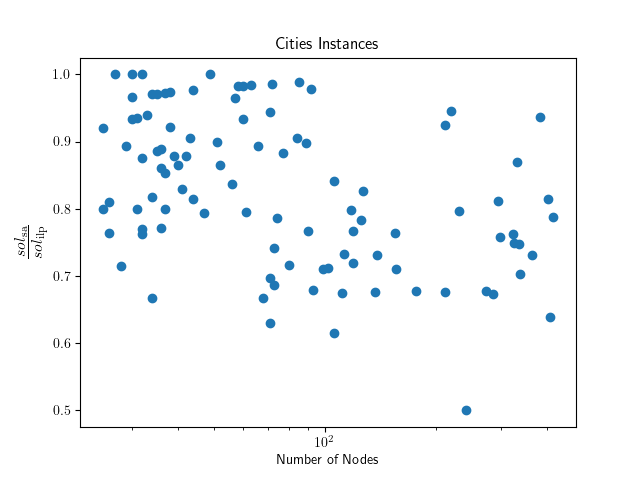
\includegraphics[width=270px]{value_sa_vs_ilp}
\end{frame}

\begin{frame}{Laufzeit ILP vs. SA}
    \centering
    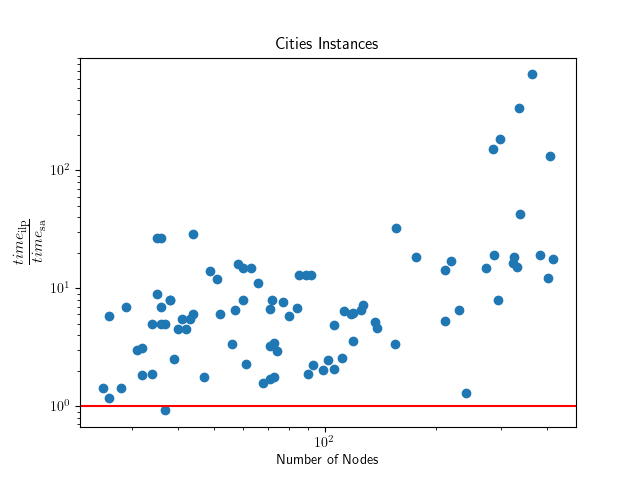
\includegraphics[width=270px]{time_ilp_vs_sa}
\end{frame}

\begin{frame}{Laufzeit mit/ohne Callback-Heuristik}
    \centering
    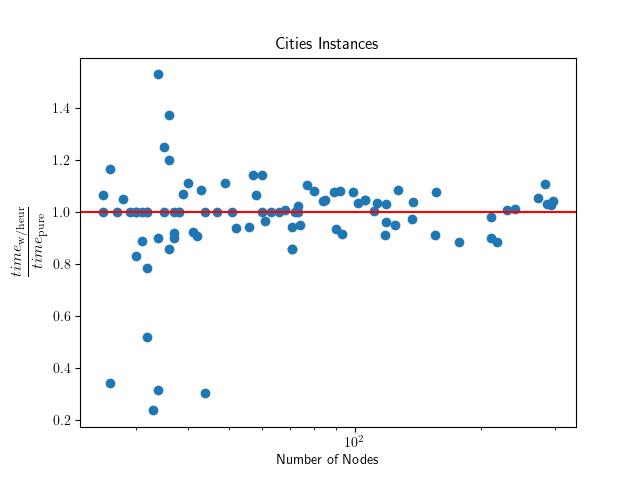
\includegraphics[width=270px]{time_heuristic_vs_pure}
\end{frame}

\begin{frame}{Laufzeit verschiedener Parameter}
    \centering
    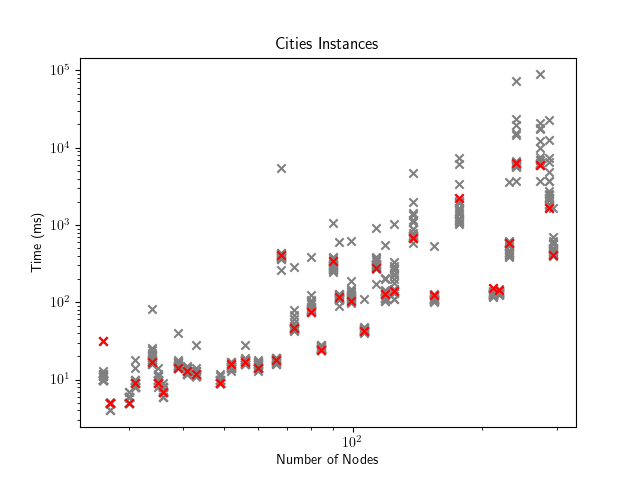
\includegraphics[width=270px]{time_ilp_parameters}
\end{frame}

\end{document}